\documentclass[11pt]{article}
\usepackage{amsmath, amssymb, physics, mathtools, bm}
\usepackage{tikz}
\usetikzlibrary{decorations.markings, decorations.pathmorphing, decorations.pathreplacing, arrows.meta}
\usepackage[margin=2.3cm]{geometry}
\usepackage{siunitx, booktabs, hyperref}
\usepackage{braket}

\newcommand{\de}{\mathrm{d}}
\newcommand{\GeV}{\,\mathrm{GeV}}
\newcommand{\MeV}{\,\mathrm{MeV}}
\newcommand{\fm}{\,\mathrm{fm}}

\title{B4 Sub-Atomic Physics --- Model Solutions, 2016}
\author{}
\date{}

\begin{document}
\maketitle

\section*{Question 1 --- Neutron structure, decay and kinematics}

\textbf{Problem.} Quark composition, spin, multiplet count of the neutron; constituent-quark estimate of $m_n$ from a uniform sphere of radius $R=1.5\fm$; neutron $\beta$-decay diagram; absence of proton decay; minimum and maximum electron energies in $n\to p\,e^-\bar\nu_e$; conversion of the free-neutron lifetime to a width.

\subsection*{Quark content / spin / multiplet}

Neutron $= udd$, spin $J = 1/2$, in the $J^P = 1/2^+$ baryon octet:
\[
\boxed{\;udd,\quad J=\tfrac12,\quad 8 \text{ hadrons in the multiplet}\;}
\]

\subsection*{(a) RMS radial position}

Uniform sphere, radius $R=1.5\fm$, density $\rho(r)= 3/(4\pi R^3)$. Mean-square radius:
\[
\langle r^2\rangle = \int_0^R r^2\,\frac{4\pi r^2}{(4/3)\pi R^3}\,\de r.
\]
Evaluate the integral:
\[
\langle r^2\rangle = \frac{3}{R^3}\int_0^R r^4\,\de r = \frac{3R^2}{5}.
\]
Take square root:
\[
\Delta r = r_{\rm rms} = R\sqrt{3/5}.
\]
Insert $R=1.5\fm$:
\[
\boxed{\;\Delta r = 1.5\sqrt{0.6}\fm = 1.16\fm\;}
\]

\subsection*{(b) Quark momentum and energy}

Heisenberg estimate, identifying $\Delta p$ with the mean momentum:
\[
\Delta p \sim \frac{\hbar}{\Delta r}.
\]
Multiply by $c$, using $\hbar c = 197.3\MeV\fm$:
\[
\Delta p\, c = \frac{197.3\MeV\fm}{1.16\fm} = 169.8\MeV.
\]
Relativistic energy with $m_q c^2 = 5\MeV$:
\[
E_q = \sqrt{(\Delta p\, c)^2 + (m_q c^2)^2}.
\]
Substitute numbers:
\[
E_q = \sqrt{169.8^2 + 5^2}\MeV = \sqrt{28857}\MeV.
\]
Evaluate:
\[
\boxed{\;E_q \approx 169.9\MeV\;}
\]

\subsection*{(c) Neutron-mass estimate and ratio}

Sum over the three constituent quarks:
\[
m_n c^2 \approx 3\,E_q = 3\times 169.9\MeV.
\]
Evaluate:
\[
\boxed{\;m_n^{\rm est} \approx 510\MeV/c^2\;}
\]
Ratio to the true neutron mass:
\[
\frac{940}{510} \approx 1.84.
\]
Improvements: include strong-interaction binding (gluon field energy, QCD potential), constituent-quark effective mass ($\sim 300\MeV$ rather than current $5\MeV$), and the colour-spin (hyperfine) interaction.

\subsection*{Neutron decay diagram}

\begin{center}
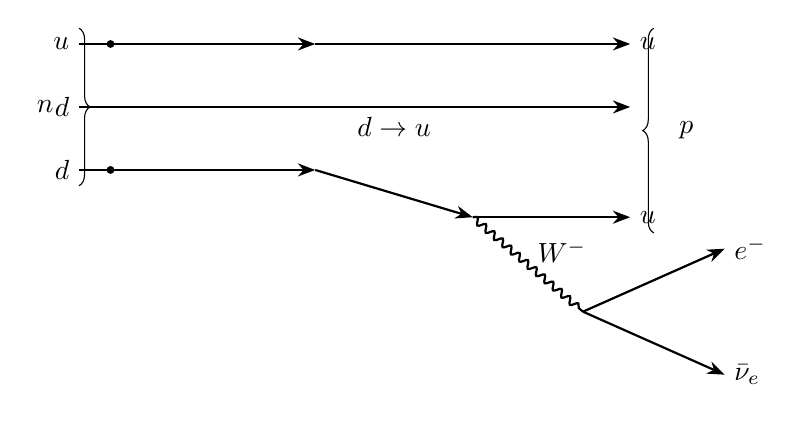
\begin{tikzpicture}[>={Stealth[length=2.2mm]}, scale=1.0]
% incoming quarks (left bracket: udd)
\draw[->,thick] (-4,1.6) -- (-1,1.6); \node[left] at (-4,1.6) {$u$};
\draw[->,thick] (-4,0.8) -- (3,0.8);  \node[left] at (-4,0.8) {$d$};
\draw[->,thick] (-4,0.0) -- (-1,0.0); \node[left] at (-4,0.0) {$d$};
% d -> u at vertex
\draw[->,thick] (-1,1.6) -- (3,1.6); \node[right] at (3,1.6) {$u$};
\draw[->,thick] (-1,0.0) -- (1,-0.6);
\node at (0.0,0.55) {$d\to u$};
\draw[->,thick] (1,-0.6) -- (3,-0.6); \node[right] at (3,-0.6) {$u$};
% W boson
\draw[decorate, decoration={snake, amplitude=1.2pt, segment length=4pt}, thick]
   (1,-0.6) -- (2.4,-1.8);
\node[above right] at (1.7,-1.3) {$W^-$};
% leptons
\draw[->,thick] (2.4,-1.8) -- (4.2,-1.0); \node[right] at (4.2,-1.0) {$e^-$};
\draw[->,thick] (2.4,-1.8) -- (4.2,-2.6); \node[right] at (4.2,-2.6) {$\bar\nu_e$};
% braces
\node[circle,fill,inner sep=1pt] (n1) at (-3.6,1.6) {};
\node[circle,fill,inner sep=1pt] (n2) at (-3.6,0.0) {};
\draw[decorate, decoration={brace, amplitude=4pt}] (-4.0,1.8) -- (-4.0,-0.2);
\node[left] at (-4.2,0.8) {$n$};
\draw[decorate, decoration={brace, amplitude=4pt, mirror}] (3.3,1.8) -- (3.3,-0.8);
\node[right] at (3.5,0.5) {$p$};
\end{tikzpicture}
\end{center}

\textbf{No proton decay.} The proton is the lightest baryon with $B=1$. Energy conservation requires
\[
m_p > m_n + m_{e^+} + m_\nu \quad \text{for } p\to n e^+\nu_e,
\]
but $m_p < m_n$, so the analogous decay is kinematically forbidden.

\subsection*{Electron energy extrema in $n\to p\,e^-\bar\nu_e$}

Three-body decay in the neutron rest frame; let $p_e$, $p_p$, $p_\nu$ denote three-momenta with $\vb p_p+\vb p_e+\vb p_\nu = 0$.

\textbf{Minimum electron energy:} the electron is at rest, $\vb p_e=0$. The proton and (massless) antineutrino balance momenta:
\[
\vb p_p = -\vb p_\nu, \qquad |\vb p_p| = |\vb p_\nu|.
\]
So the minimum is just the rest energy:
\[
\boxed{\;E_e^{\min} = m_e c^2\;}
\]

\textbf{Maximum electron energy:} the antineutrino has zero momentum (massless $\Rightarrow E_\nu=0$). Electron and proton recoil back-to-back:
\[
\vb p_p = -\vb p_e, \qquad |\vb p_p| = |\vb p_e| \equiv p.
\]
Four-momentum conservation: $E_e + E_p = m_n c^2$. Square the proton four-momentum:
\[
(m_n c^2 - E_e)^2 = (p c)^2 + (m_p c^2)^2.
\]
Use $(pc)^2 = E_e^2 - (m_e c^2)^2$:
\[
m_n^2 c^4 - 2 m_n c^2 E_e + E_e^2 = E_e^2 - m_e^2 c^4 + m_p^2 c^4.
\]
Cancel $E_e^2$:
\[
m_n^2 c^4 - 2 m_n c^2 E_e = m_p^2 c^4 - m_e^2 c^4.
\]
Solve for $E_e$:
\[
\boxed{\;E_e^{\max} = \frac{m_n^2 + m_e^2 - m_p^2}{2\,m_n}\,c^2\;}
\]

\subsection*{Decay width from lifetime}

Use $\Gamma = \hbar/\tau$ with $\tau = 15 \times 60\,\text{s} = 900\,\text{s}$:
\[
\Gamma = \frac{\hbar}{\tau} = \frac{6.582\times10^{-16}\,\text{eV\,s}}{900\,\text{s}}.
\]
Evaluate:
\[
\boxed{\;\Gamma \approx 7.3\times10^{-19}\,\text{eV}\;}
\]

\section*{Question 2 --- Light mesons and resonant production}

\textbf{Problem.} Pseudoscalar nonet of $K$ and $\pi$; Feynman diagrams and suppression factors for $\pi^+\!\to\mu^+\nu_\mu$, $K^+\!\to\mu^+\nu_\mu$, $K^+\!\to\pi^+\pi^0$; resonance cross-section ratio for $\rho^0$ vs $K^0$ produced in $\pi^+\pi^-$ at $E=249$ and $250\MeV$ per beam; pion radius of curvature in a $1\,\text{T}$ field.

\subsection*{Pseudoscalar meson nonet}

Axes: third isospin component $I_3$ (charge $Q = I_3 + Y/2$) and strangeness $S$.

\begin{center}
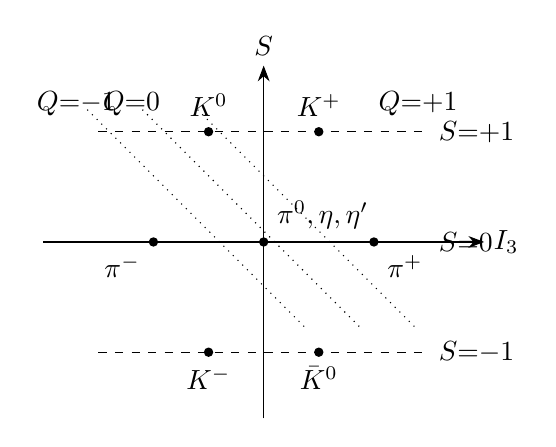
\begin{tikzpicture}[>={Stealth[length=2mm]}, scale=1.4]
% axes
\draw[->] (-2.0,0) -- (2.0,0) node[right] {$I_3$};
\draw[->] (0,-1.6) -- (0,1.6) node[above] {$S$};
% lattice points
\node[circle,fill,inner sep=1.2pt,label=above:{$K^0$}]      (K0) at (-0.5, 1) {};
\node[circle,fill,inner sep=1.2pt,label=above:{$K^+$}]      (Kp) at ( 0.5, 1) {};
\node[circle,fill,inner sep=1.2pt,label=below left:{$\pi^-$}]  (pim) at (-1.0, 0) {};
\node[circle,fill,inner sep=1.2pt,label=above right:{$\pi^0,\eta,\eta'$}]  (pi0) at ( 0.0, 0) {};
\node[circle,fill,inner sep=1.2pt,label=below right:{$\pi^+$}] (pip) at ( 1.0, 0) {};
\node[circle,fill,inner sep=1.2pt,label=below:{$K^-$}]      (Km) at (-0.5,-1) {};
\node[circle,fill,inner sep=1.2pt,label=below:{$\bar K^0$}] (K0b) at ( 0.5,-1) {};
% S = +1 line
\draw[dashed] (-1.5, 1) -- (1.5, 1) node[right] {$S{=}{+}1$};
\draw[dashed] (-1.5, 0) -- (1.5, 0) node[right] {$S{=}0$};
\draw[dashed] (-1.5,-1) -- (1.5,-1) node[right] {$S{=}{-}1$};
% constant-Q diagonals (Q = I_3 + (B+S)/2 = I_3 + S/2 for mesons)
\draw[dotted] (-1.6, 1.2) -- (0.4,-0.8); \node at (-1.7, 1.25) {$Q{=}{-}1$};
\draw[dotted] (-1.1, 1.2) -- (0.9,-0.8); \node at (-1.2, 1.25) {$Q{=}0$};
\draw[dotted] (-0.6, 1.2) -- (1.4,-0.8); \node at (1.4, 1.25)  {$Q{=}{+}1$};
\end{tikzpicture}
\end{center}

Nine states: triplet $\pi^{\pm,0}$ and singlets $\eta,\eta'$ at $S=0$; $(K^+,K^0)$ at $S=+1$; $(K^-,\bar K^0)$ at $S=-1$.

\subsection*{Feynman diagrams and suppression factors}

\textbf{$\pi^+\to\mu^+\nu_\mu$} ($\bar d u$ annihilation, $V_{ud}$):

\begin{center}
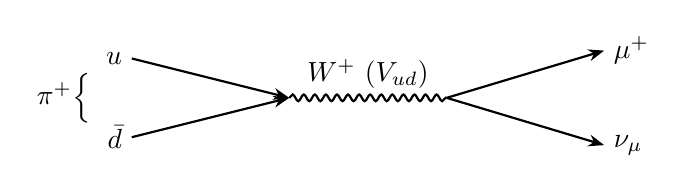
\begin{tikzpicture}[>={Stealth[length=2mm]}, scale=1.0]
\draw[->,thick] (-3,0.5) -- (-1,0.0); \node[left] at (-3,0.5) {$u$};
\draw[->,thick] (-3,-0.5) -- (-1,0.0); \node[left] at (-3,-0.5) {$\bar d$};
\node[left] at (-3.4,0.0) {$\pi^+\Bigl\{$};
\draw[decorate, decoration={snake, amplitude=1.2pt, segment length=4pt}, thick] (-1,0.0) -- (1,0.0);
\node[above] at (0,0.0) {$W^+$ ($V_{ud}$)};
\draw[->,thick] (1,0.0) -- (3,0.6);  \node[right] at (3,0.6)  {$\mu^+$};
\draw[->,thick] (1,0.0) -- (3,-0.6); \node[right] at (3,-0.6) {$\nu_\mu$};
\end{tikzpicture}
\end{center}

\textbf{$K^+\to\mu^+\nu_\mu$} ($\bar s u$ annihilation, $V_{us}$):

\begin{center}
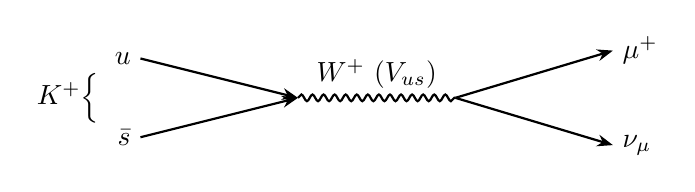
\begin{tikzpicture}[>={Stealth[length=2mm]}, scale=1.0]
\draw[->,thick] (-3,0.5) -- (-1,0.0); \node[left] at (-3,0.5) {$u$};
\draw[->,thick] (-3,-0.5) -- (-1,0.0); \node[left] at (-3,-0.5) {$\bar s$};
\node[left] at (-3.4,0.0) {$K^+\Bigl\{$};
\draw[decorate, decoration={snake, amplitude=1.2pt, segment length=4pt}, thick] (-1,0.0) -- (1,0.0);
\node[above] at (0,0.0) {$W^+$ ($V_{us}$)};
\draw[->,thick] (1,0.0) -- (3,0.6);  \node[right] at (3,0.6)  {$\mu^+$};
\draw[->,thick] (1,0.0) -- (3,-0.6); \node[right] at (3,-0.6) {$\nu_\mu$};
\end{tikzpicture}
\end{center}

\textbf{$K^+\to\pi^+\pi^0$} (spectator $u$; $s\to u$ via $W^+\to u\bar d$, $V_{us}$):

\begin{center}
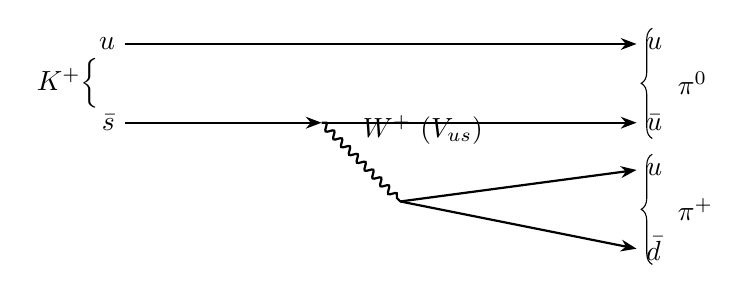
\begin{tikzpicture}[>={Stealth[length=2mm]}, scale=1.0]
\draw[->,thick] (-3.5,1.0) -- (3,1.0);
\node[left]  at (-3.5,1.0) {$u$};
\node[right] at (3,1.0)    {$u$};
\draw[->,thick] (-3.5,0.0) -- (-1,0.0);
\node[left] at (-3.5,0.0) {$\bar s$};
\draw[->,thick] (-1,0.0) -- (3,0.0);
\node[right] at (3,0.0) {$\bar u$};
\draw[decorate, decoration={snake, amplitude=1.2pt, segment length=4pt}, thick] (-1,0.0) -- (0,-1.0);
\node[above right] at (-0.6,-0.4) {$W^+$ ($V_{us}$)};
\draw[->,thick] (0,-1.0) -- (3,-0.6); \node[right] at (3,-0.6) {$u$};
\draw[->,thick] (0,-1.0) -- (3,-1.6); \node[right] at (3,-1.6) {$\bar d$};
\node[left] at (-3.7,0.5) {$K^+\Bigl\{$};
\draw[decorate, decoration={brace, amplitude=4pt, mirror}] (3.2,1.2) -- (3.2,-0.2); \node[right] at (3.4,0.5) {$\pi^0$};
\draw[decorate, decoration={brace, amplitude=4pt, mirror}] (3.2,-0.4) -- (3.2,-1.8); \node[right] at (3.4,-1.1) {$\pi^+$};
\end{tikzpicture}
\end{center}

\textbf{Suppression factors.}
\begin{itemize}
\item $\pi^+\to\mu^+\nu$ vs.\ $K^+\to\mu^+\nu$: both share the same leptonic helicity factor $(m_\mu/m_P)^2(1-m_\mu^2/m_P^2)^2$ and a CKM factor ($V_{ud}^2$ vs $V_{us}^2$). The pion partial width is suppressed by the much smaller phase space available, $\Gamma\propto m_P\,(m_\mu/m_P)^2(1-m_\mu^2/m_P^2)^2$, which is dominated by $m_P$. So pion-decay is \emph{phase-space suppressed} relative to kaon-decay.
\item $K^+$ decays vs.\ $\pi^+\to\mu^+\nu$: kaon decays are Cabibbo-suppressed by $|V_{us}|^2 = \sin^2\theta_C\approx 0.05$ (vs.\ $|V_{ud}|^2\approx\cos^2\theta_C$). $K^+\to\mu^+\nu$ is additionally helicity-suppressed by $(m_\mu/m_K)^2$ relative to $K^+\to\pi^+\pi^0$.
\end{itemize}

\subsection*{(a) $\sigma(\rho^0)/\sigma(K^0)$ at $E=2\times 249\MeV = 498\MeV$}

Use the Breit-Wigner with $E_{\rm cm}=498\MeV = m_K c^2$.

For $K^0$ ($J=0$, on resonance, $B_{\rm in}=B_{\rm out}=0.69$, $m_K=498$, $\Gamma_K=7.4\times 10^{-12}\MeV$):
\[
\sigma_K \propto (2\cdot 0+1)\,\frac{(0.69)^2\,\Gamma_K^2}{0 + m_K^2\,\Gamma_K^2}.
\]
Cancel $\Gamma_K^2$:
\[
\sigma_K \propto \frac{(0.69)^2}{m_K^2} = \frac{0.4761}{498^2}\MeV^{-2}.
\]
Evaluate:
\[
\sigma_K \propto \frac{0.4761}{2.480\times 10^5} = 1.920\times 10^{-6}\MeV^{-2}.
\]

For $\rho^0$ ($J=1$, $B_{\rm in}B_{\rm out}=1$, $m_\rho=769$, $\Gamma_\rho=147\MeV$, $E=498$):
\[
(E^2 - m_\rho^2)^2 = (498^2 - 769^2)^2\MeV^4.
\]
Insert squares:
\[
(E^2 - m_\rho^2)^2 = (2.480\times 10^5 - 5.914\times 10^5)^2 = (3.434\times 10^5)^2.
\]
Evaluate:
\[
(E^2 - m_\rho^2)^2 = 1.179\times 10^{11}\MeV^4.
\]
And:
\[
E^2\Gamma_\rho^2 = (498)^2(147)^2 = 2.480\times 10^5 \times 2.161\times 10^4 = 5.359\times 10^{9}\MeV^4.
\]
Sum:
\[
D_\rho = 1.179\times 10^{11} + 5.359\times 10^9 = 1.233\times 10^{11}\MeV^4.
\]
Numerator:
\[
N_\rho = 3 \times 1 \times \Gamma_\rho^2 = 3 \times 2.161\times 10^4 = 6.483\times 10^4\MeV^2.
\]
Hence:
\[
\sigma_\rho \propto \frac{6.483\times 10^4}{1.233\times 10^{11}} = 5.258\times 10^{-7}\MeV^{-2}.
\]
Take the ratio:
\[
\frac{\sigma_\rho}{\sigma_K} = \frac{5.258\times 10^{-7}}{1.920\times 10^{-6}}.
\]
Evaluate:
\[
\boxed{\;\frac{\sigma_\rho}{\sigma_K}\bigg|_{498\MeV} \approx 0.27\;}
\]

\subsection*{(b) Beam energy raised to $250\MeV$ ($E=500\MeV$)}

Now $K^0$ is just off resonance; redo the denominator for $K$:
\[
(E^2-m_K^2)^2 = (500^2 - 498^2)^2 = (1.996\times 10^3)^2 = 3.984\times 10^{6}\MeV^4.
\]
And:
\[
E^2\Gamma_K^2 = 2.500\times 10^5 \times (7.4\times 10^{-12})^2 = 1.369\times 10^{-17}\MeV^4.
\]
The width-squared term is negligible:
\[
D_K \approx 3.984\times 10^{6}\MeV^4.
\]
Numerator $N_K = 1\times 0.4761 \times \Gamma_K^2 = 0.4761\times 5.476\times 10^{-23}\MeV^4 = 2.607\times 10^{-23}\MeV^4$:
\[
\sigma_K \propto \frac{2.607\times 10^{-23}}{3.984\times 10^{6}} = 6.54\times 10^{-30}\MeV^{-2}.
\]

For $\rho^0$ at $E=500$:
\[
(E^2-m_\rho^2)^2 = (2.500\times 10^5 - 5.914\times 10^5)^2 = (3.414\times 10^5)^2 = 1.165\times 10^{11}\MeV^4.
\]
$E^2\Gamma_\rho^2 = 2.500\times 10^5\times 2.161\times 10^4 = 5.402\times 10^9$. Sum:
\[
D_\rho = 1.165\times 10^{11} + 5.402\times 10^9 = 1.219\times 10^{11}\MeV^4.
\]
\[
\sigma_\rho \propto \frac{6.483\times 10^4}{1.219\times 10^{11}} = 5.319\times 10^{-7}\MeV^{-2}.
\]
Ratio:
\[
\frac{\sigma_\rho}{\sigma_K}\bigg|_{500\MeV} = \frac{5.319\times 10^{-7}}{6.54\times 10^{-30}}.
\]
Evaluate:
\[
\boxed{\;\frac{\sigma_\rho}{\sigma_K}\bigg|_{500\MeV} \approx 8\times 10^{22}\;}
\]
A $2\MeV$ shift off the $K^0$ peak collapses the cross-section by $\sim 23$ orders of magnitude: $\Gamma_K\sim 10^{-12}\MeV$ requires energy resolution $\Delta E\lesssim \Gamma_K \sim 10^{-12}\MeV$, far beyond any beam, so resonant $K^0$ production via $\pi^+\pi^-$ is impractical.

\subsection*{(c) Radius of curvature of the pion}

Pion mass $m_\pi = 139.57\MeV/c^2$, $E_\pi=249\MeV$:
\[
(p_\pi c)^2 = E^2 - (m_\pi c^2)^2 = 249^2 - 139.57^2.
\]
Evaluate squares:
\[
(p_\pi c)^2 = 62001 - 19480 = 42521\MeV^2.
\]
Take square root:
\[
p_\pi c = 206.2\MeV.
\]
Radius of curvature, $r = p/(qB)$, i.e.\ $r = (pc)/(qBc)$ with $qB=1\,\text{eV\,s\,m}^{-2}$:
\[
r = \frac{2.062\times 10^{8}\,\text{eV}}{(1\,\text{eV\,s\,m}^{-2})(3\times 10^8\,\text{m\,s}^{-1})}.
\]
Evaluate:
\[
\boxed{\;r \approx 0.69\,\text{m}\;}
\]

\section*{Question 3 --- Fusion, fission and moderation}

\textbf{Problem.} pp-fusion start; total H consumed by the Sun and remaining lifetime; SEMF term-by-term; energy released and uranium burned in $^{235}$U fission; collisions to thermalise neutrons in graphite.

\subsection*{(a) Initial $pp$-fusion step}

\[
\boxed{\;p + p \;\longrightarrow\; {}^2_1\!H + e^+ + \nu_e,\qquad Q \approx 0.42\MeV\;}
\]

\subsection*{(b) Hydrogen burned to date and time remaining}

Energy delivered to the Sun's photosphere per chain (annihilation included, neutrinos lost):
\[
E_{\rm chain} = Q + 2\times 1.02\MeV - 2\times 0.26\MeV.
\]
Evaluate:
\[
E_{\rm chain} = 24.68 + 2.04 - 0.52 = 26.20\MeV.
\]
Per H nucleus consumed (4 H per chain):
\[
E_H = E_{\rm chain}/4 = 6.55\MeV.
\]
Time elapsed:
\[
t = 4.6\times 10^9\,\text{yr} \times 3.156\times 10^7\,\text{s\,yr}^{-1} = 1.452\times 10^{17}\,\text{s}.
\]
Total energy emitted:
\[
E_{\rm tot} = L_\odot\, t = 3.86\times 10^{26}\,\text{W}\times 1.452\times 10^{17}\,\text{s}.
\]
Evaluate:
\[
E_{\rm tot} = 5.604\times 10^{43}\,\text{J}.
\]
Convert to MeV ($1\MeV=1.602\times 10^{-13}\,\text{J}$):
\[
E_{\rm tot} = \frac{5.604\times 10^{43}}{1.602\times 10^{-13}} = 3.499\times 10^{56}\MeV.
\]
Number of H burned:
\[
N_H^{\rm burned} = \frac{E_{\rm tot}}{E_H} = \frac{3.499\times 10^{56}}{6.55}.
\]
Evaluate:
\[
\boxed{\;N_H^{\rm burned} \approx 5.34\times 10^{55}\;}
\]
Remaining H: $9\times 10^{56} - 5.34\times 10^{55} = 8.47\times 10^{56}$. Time remaining at constant luminosity:
\[
t_{\rm rem} = \frac{N_H^{\rm rem}}{N_H^{\rm burned}}\,t = \frac{8.47\times 10^{56}}{5.34\times 10^{55}}\times 4.6\times 10^9\,\text{yr}.
\]
Evaluate:
\[
\boxed{\;t_{\rm rem} \approx 7.3\times 10^{10}\,\text{yr}\;}
\]

\subsection*{(c) SEMF terms}

\begin{itemize}
\item $Z(m_p+m_e)$: rest mass of $Z$ protons plus their atomic electrons (atomic-mass convention).
\item $(A-Z)m_n$: rest mass of $N=A-Z$ neutrons.
\item $-a_v A$ (\textbf{volume}, attractive): each nucleon feels short-range strong attraction from a roughly fixed number of neighbours; binding energy is therefore extensive in $A$.
\item $+a_s A^{2/3}$ (\textbf{surface}, reduces binding): surface nucleons have fewer neighbours; the surface term subtracts the over-counting in the volume term, scaling as the area.
\item $+a_c Z^2/A^{1/3}$ (\textbf{Coulomb}, reduces binding): electrostatic repulsion between $Z$ protons in a sphere of radius $\propto A^{1/3}$ gives self-energy $\propto Z^2/A^{1/3}$.
\item $+a_a (Z-A/2)^2/A$ (\textbf{asymmetry/symmetry}, reduces binding when $N\ne Z$): Pauli exclusion + isospin symmetry of the strong force favour $N=Z$; converting protons to neutrons (or vice versa) costs Fermi-level kinetic energy.
\item $\pm a_p A^{-1/2}$ (\textbf{pairing}): like-nucleon pairs couple to $J=0$ for extra binding; sign $+$ for odd-odd (less bound), $0$ for odd-$A$, $-$ for even-even (more bound).
\end{itemize}

\subsection*{(d) Energy released per $^{235}$U fission and annual mass burned}

Reaction: $n + {}^{235}_{92}\!\text{U} \to {}^{92}_{37}\!\text{Rb} + {}^{140}_{55}\!\text{Cs} + 4n$. Charge ($92=37+55$) and baryon ($235+1=92+140+4$) conserved. The mass-difference reduces (as derived above) to
\[
Q = B(^{92}\!\text{Rb}) + B(^{140}\!\text{Cs}) - B(^{235}\!\text{U}),
\]
with binding energy $B(Z,A) = a_v A - a_s A^{2/3} - a_c Z^2/A^{1/3} - a_a(Z-A/2)^2/A \mp a_p A^{-1/2}$.

\textbf{$^{235}$U} ($Z=92$, $A=235$, odd-$A$ so pairing $=0$):
\[
a_v A = 15.56 \times 235 = 3656.6\MeV.
\]
\[
A^{2/3} = 235^{2/3} = 38.08;\quad a_s A^{2/3} = 17.23\times 38.08 = 656.1\MeV.
\]
\[
A^{1/3} = 6.171;\quad a_c Z^2/A^{1/3} = 0.697\times 8464/6.171 = 956.0\MeV.
\]
\[
(Z-A/2)^2 = (92-117.5)^2 = 649.25;\quad a_a(\cdot)/A = 93.14\times 649.25/235 = 257.3\MeV.
\]
Sum:
\[
B(^{235}\!\text{U}) = 3656.6 - 656.1 - 956.0 - 257.3 = 1787.2\MeV.
\]

\textbf{$^{92}$Rb} ($Z=37$, $A=92$, $N=55$, odd-odd $\Rightarrow$ pairing $+12/\sqrt{A}$):
\[
a_v A = 15.56\times 92 = 1431.5\MeV.
\]
\[
A^{2/3} = 92^{2/3} = 20.38;\quad a_s A^{2/3} = 17.23\times 20.38 = 351.1\MeV.
\]
\[
A^{1/3} = 4.514;\quad a_c Z^2/A^{1/3} = 0.697\times 1369/4.514 = 211.4\MeV.
\]
\[
(Z-A/2)^2 = (37-46)^2 = 81;\quad a_a\cdot 81/92 = 93.14\times 0.880 = 82.0\MeV.
\]
\[
a_p A^{-1/2} = 12/\sqrt{92} = 1.25\MeV \quad (\text{odd-odd: subtract}).
\]
Sum:
\[
B(^{92}\!\text{Rb}) = 1431.5 - 351.1 - 211.4 - 82.0 - 1.25 = 785.7\MeV.
\]

\textbf{$^{140}$Cs} ($Z=55$, $A=140$, $N=85$, odd-odd):
\[
a_v A = 15.56\times 140 = 2178.4\MeV.
\]
\[
A^{2/3} = 140^{2/3} = 26.96;\quad a_s A^{2/3} = 17.23\times 26.96 = 464.5\MeV.
\]
\[
A^{1/3} = 5.192;\quad a_c Z^2/A^{1/3} = 0.697\times 3025/5.192 = 406.1\MeV.
\]
\[
(Z-A/2)^2 = (55-70)^2 = 225;\quad a_a\cdot 225/140 = 93.14\times 1.607 = 149.7\MeV.
\]
\[
a_p A^{-1/2} = 12/\sqrt{140} = 1.01\MeV.
\]
Sum:
\[
B(^{140}\!\text{Cs}) = 2178.4 - 464.5 - 406.1 - 149.7 - 1.01 = 1157.1\MeV.
\]

Combine:
\[
Q = 785.7 + 1157.1 - 1787.2.
\]
Evaluate:
\[
\boxed{\;Q \approx 156\MeV\;}
\]

Per fission in joules:
\[
Q = 155.6\MeV \times 1.602\times 10^{-13}\,\text{J/MeV} = 2.493\times 10^{-11}\,\text{J}.
\]
Fission rate at $P=100\,\text{MW}=10^8\,\text{W}$:
\[
\dot N = \frac{P}{Q} = \frac{10^{8}}{2.493\times 10^{-11}} = 4.01\times 10^{18}\,\text{s}^{-1}.
\]
Per year ($3.156\times 10^7\,\text{s}$):
\[
N_{\rm yr} = 4.01\times 10^{18}\times 3.156\times 10^7.
\]
Evaluate:
\[
\boxed{\;N_{\rm yr} \approx 1.27\times 10^{26}\,\text{atoms\,yr}^{-1}\;}
\]
Mass per atom $= 235\,\text{u} \times 1.661\times 10^{-27}\,\text{kg} = 3.903\times 10^{-25}\,\text{kg}$:
\[
m_{\rm yr} = 1.266\times 10^{26}\times 3.903\times 10^{-25}\,\text{kg}.
\]
Evaluate:
\[
\boxed{\;m_{\rm yr} \approx 49.4\,\text{kg} = 4.94\times 10^4\,\text{g}\;}
\]

\subsection*{(e) Number of elastic collisions to thermalise}

Per collision energy ratio:
\[
f \equiv \frac{E_f}{E_i} = \frac{m_C^2 + m_n^2}{(m_C+m_n)^2}.
\]
Insert $m_n=0.94\GeV$, $m_C=11.18\GeV$:
\[
f = \frac{(11.18)^2 + (0.94)^2}{(12.12)^2} = \frac{124.99 + 0.884}{146.89}.
\]
Evaluate:
\[
f = \frac{125.87}{146.89} = 0.857.
\]
After $N$ collisions $E_N = E_0\, f^N$. Required reduction:
\[
\frac{E_N}{E_0} = \frac{0.025\,\text{eV}}{2\times 10^6\,\text{eV}} = 1.25\times 10^{-8}.
\]
Solve for $N$:
\[
N = \frac{\ln(1.25\times 10^{-8})}{\ln 0.857} = \frac{-18.20}{-0.1542}.
\]
Evaluate:
\[
\boxed{\;N \approx 118\;}
\]

\section*{Question 4 --- $W$ and $Z$ widths and the fourth generation}

\textbf{Problem.} List $W,Z$ first-generation decays; compute lepton-pair and quark-pair branching ratios; deduce the number of fermion pairs in the $W$ width; mass constraints on a fourth generation; relate the $W$ width to the $W/Z$ cross-section ratio; predict $\Gamma_W$, $\Gamma_Z$ and the cross-section ratio with a fourth generation contributing; compare with CDF and LEP precision.

\subsection*{(a) First-generation decays and branching ratios}

\textbf{$Z$ (first generation):} $Z\to e^+e^-,\;\nu_e\bar\nu_e,\;u\bar u,\;d\bar d$.

\textbf{$W^+$ (first generation):} $W^+\to e^+\nu_e,\;u\bar d$.

Counting open channels for the full $W$ ($t$-quark too heavy): three lepton flavours $(e\nu_e,\mu\nu_\mu,\tau\nu_\tau)$ and two quark Cabibbo doublets $(u\bar d,c\bar s)$ each in 3 colours. Equal partial widths:
\[
N_{\rm channels} = 3 \;+\; 2\times 3 = 9.
\]
Hence:
\[
\boxed{\;\text{BR}(W\to\ell\nu_\ell) = \tfrac{1}{9}\approx 11.1\%,\qquad \text{BR}(W\to q\bar q')_{\rm summed\ colour} = \tfrac{3}{9}\approx 33.3\%\;}
\]

\subsection*{(b) Number of distinguishable fermion pairs in $\Gamma_W$}

Equal partial widths, so
\[
N_{\rm pairs} = \frac{\Gamma_W^{\rm tot}}{\Gamma(W\to e\nu)} = \frac{2085}{232}.
\]
Evaluate:
\[
\boxed{\;N_{\rm pairs} \approx 9\;}
\]
Consistent with three lepton flavours and two colour-tripled quark doublets; no fourth generation in $W$ decay.

\subsection*{(c) Mass constraints from $W,Z$ widths}

The measured widths leave no room for new on-shell decays. Therefore each fourth-generation pair must be kinematically forbidden:
\[
\boxed{\;m_T+m_B > m_W,\qquad m_\sigma + m_N > m_W\;}
\]
\[
\boxed{\;2m_T,\,2m_B,\,2m_\sigma,\,2m_N > m_Z\;}
\]
i.e.\ each new fermion mass $> m_Z/2 \approx 45.6\GeV$, with the additional pair-sum constraints from $W$ decay.

\subsection*{(d) Indirect determination of $\Gamma_W$}

At the resonance peak ($E=m$), with $J=1$ for both $W$ and $Z$, the Breit-Wigner reduces to
\[
\sigma(m) = K\,(2J+1)\,\frac{B_{\rm in}B_{\rm out}\,\Gamma_{\rm tot}^2}{m^2\,\Gamma_{\rm tot}^2} = 3K\,\frac{\Gamma_{\rm in}\Gamma_{\rm out}}{m^2\,\Gamma_{\rm tot}^2}.
\]
Define the measured ratio:
\[
R \equiv \frac{\sigma(W\to\ell\nu)}{\sigma(Z\to\ell\ell)}.
\]
Substitute the peak expressions ($K$ cancels by assumption):
\[
R = \frac{\Gamma_{\rm in}^W\,\Gamma_{\rm out}^W}{m_W^2\,\Gamma_W^2}\,\bigg/\,\frac{\Gamma_{\rm in}^Z\,\Gamma_{\rm out}^Z}{m_Z^2\,\Gamma_Z^2}.
\]
Rearrange for $\Gamma_W^2$:
\[
\Gamma_W^2 = \frac{\Gamma_{\rm in}^W\,\Gamma_{\rm out}^W\,m_Z^2\,\Gamma_Z^2}{R\,\Gamma_{\rm in}^Z\,\Gamma_{\rm out}^Z\,m_W^2}.
\]
Take square root:
\[
\boxed{\;\Gamma_W = \frac{m_Z\,\Gamma_Z}{m_W}\,\sqrt{\frac{\Gamma_{\rm in}^W\,\Gamma_{\rm out}^W}{R\,\Gamma_{\rm in}^Z\,\Gamma_{\rm out}^Z}}\;}
\]

\subsection*{(e) Effect of a fourth generation of leptons on $\Gamma_W,\Gamma_Z$ and $R$}

Per-flavour partial widths:
\[
\Gamma(Z\to\nu\bar\nu)|_{\rm flavour} = \frac{501}{3} = 167\MeV,\qquad \Gamma(Z\to\ell^+\ell^-)|_{\rm flavour} = 84\MeV.
\]
Add one fourth generation (one $\nu_4$, one $\ell_4$):
\[
\Gamma_Z' = 2495 + 167 + 84 = 2746\MeV.
\]
Boxed:
\[
\boxed{\;\Gamma_Z' = 2746\MeV\;}
\]
For $W$, add one extra lepton-pair channel of partial width $232\MeV$:
\[
\Gamma_W' = 2085 + 232 = 2317\MeV.
\]
Boxed:
\[
\boxed{\;\Gamma_W' = 2317\MeV\;}
\]

Ratio sensitivity. From (d), at fixed standard-model partial widths,
\[
R \;\propto\; \frac{1/\Gamma_W^2}{1/\Gamma_Z^2} = \frac{\Gamma_Z^2}{\Gamma_W^2}.
\]
So:
\[
\frac{R'}{R} = \left(\frac{\Gamma_Z'}{\Gamma_Z}\right)^2 \bigg/\left(\frac{\Gamma_W'}{\Gamma_W}\right)^2.
\]
Insert numbers:
\[
\frac{\Gamma_Z'}{\Gamma_Z} = \frac{2746}{2495} = 1.1006;\qquad \frac{\Gamma_W'}{\Gamma_W} = \frac{2317}{2085} = 1.1113.
\]
Square and divide:
\[
\frac{R'}{R} = \frac{(1.1006)^2}{(1.1113)^2} = \frac{1.2114}{1.2350} = 0.9809.
\]
Fractional change:
\[
\boxed{\;\frac{\Delta R}{R} = -1.91\%\;}
\]

\subsection*{(f) Significance at CDF and LEP}

CDF $\sigma$-ratio (1.9\% precision):
\[
n_\sigma^{\rm CDF} = \frac{|\Delta R/R|}{0.019} = \frac{0.0191}{0.019}.
\]
Evaluate:
\[
\boxed{\;n_\sigma^{\rm CDF} \approx 1.0\,\sigma\;}
\]

LEP $\Gamma_Z$ (2.3 MeV precision):
\[
n_\sigma^{\rm LEP} = \frac{\Delta\Gamma_Z}{2.3\MeV} = \frac{2746-2495}{2.3} = \frac{251}{2.3}.
\]
Evaluate:
\[
\boxed{\;n_\sigma^{\rm LEP} \approx 109\,\sigma\;}
\]
LEP rules out a low-mass fourth generation overwhelmingly; CDF, by contrast, has only marginal sensitivity through the cross-section ratio.

\end{document}
